\documentclass[usenames,dvipsnames]{beamer}

\usepackage[nolist,nohyperlinks]{acronym}
\usepackage{color}
\usepackage{listings}
\usepackage[absolute,overlay]{textpos}
\usepackage{tikz}
\usepackage{tikz-uml}
\usepackage{xcolor}

\usetikzlibrary{decorations.pathreplacing}

% https://tex.stackexchange.com/a/146991
\tikzset{
  invisible/.style={opacity=0,text opacity=0},
  visible on/.style={alt={#1{}{invisible}}},
  alt/.code args={<#1>#2#3}{
    \alt<#1>{\pgfkeysalso{#2}}{\pgfkeysalso{#3}}
  },
}

\definecolor{mygreen}{HTML}{95cf95}

\newacro{BP7}[BP]{Bundle Protocol Version 7}
\newacro{BP}{Bundle Protocol}
\newacro{DTN}{Delay / Disruption-tolerant Networking}


\usetheme{default}
\usecolortheme{dove}
\beamertemplatenavigationsymbolsempty

\title{DTN7}
\subtitle{An Open-Source Disruption-tolerant Networking Implementation of Bundle Protocol 7}
\author{Alvar Penning, Lars Baumgärtner, Jonas Höchst,\\
  Artur Sterz, Mira Mezini, Bernd Freisleben}
% \institute{Distributed Systems Group \\ Philipps University of Marburg}
\date{AdHoc-Now 2019}
\titlegraphic{
  
\includegraphics[width=0.35\linewidth]{include/umr-logo}~
  
\includegraphics[width=0.35\linewidth]{include/tud-logo}}

\begin{document}

\begin{frame}
  \titlepage
\end{frame}

% \begin{frame}
%   \frametitle{Outline}
%   \tableofcontents
% \end{frame}

\section{\acf{DTN}}

\begin{frame}
  \frametitle{\acf{DTN}}

  \begin{columns}
  \column{0.6\textwidth}
  \begin{itemize}
  \item In \acs{DTN}, data is transmitted in a store-carry-forward fashion
    \begin{itemize}
    \item Hop-by-hop transport
    \item Opportunistic or scheduled contacts to neighbors
    \item Allows large time window between two transmissions
    \end{itemize}

  \item Useful if there is no reliable connection
    \begin{itemize}
    \item Environmental monitoring in remote areas
    \item Destroyed telecommunication infrastructure
    \item Internet access is blocked
    \end{itemize}
  \end{itemize}

  \column{0.4\textwidth}
  \end{columns}

  \begin{textblock*}{0.4\textwidth}(0.7\textwidth,1.75cm)
    \includegraphics<2>[width=\linewidth,height=\textheight,keepaspectratio]{include/dtn-example-1}
    \includegraphics<3>[width=\linewidth,height=\textheight,keepaspectratio]{include/dtn-example-2}
    \includegraphics<4>[width=\linewidth,height=\textheight,keepaspectratio]{include/dtn-example-3}
    \includegraphics<5>[width=\linewidth,height=\textheight,keepaspectratio]{include/dtn-example-4}
  \end{textblock*}
\end{frame}

\begin{frame}
  \frametitle{DTN7}

  This brings us to DTN7\dots

  \begin{itemize}
  \item Free and open-source \acs{DTN} software
  \item Written in the Go programming language
  \item Modularized design, easy to extend
  \item Implementation of the recently released \acf{BP}
  \end{itemize}
\end{frame}

\section{\acf{DTN}}

\subsection{Introduction}

\begin{frame}
  \frametitle{\acf{BP7}}

  \begin{itemize}
  \item Describes both a \acs{DTN} architecture and protocol
  \item Still in development, but nearly finished
  \item Latest draft (version 14) was released on 04.08.2019
  \item Aims to obsolete Bundle Protocol Version 6, RFC 5050
  \end{itemize}
\end{frame}

\subsection{Nodes and Endpoints}

\begin{frame}
  \frametitle{Nodes and Endpoints}

  \begin{itemize}
  \item Nodes are identified by an Endpoint ID (URI), e.g., \texttt{dtn:node}
  \item A node might be addressed by multiple Endpoint IDs
  \item An Endpoint ID might represent multiple nodes
  \end{itemize}

  \begin{figure}
    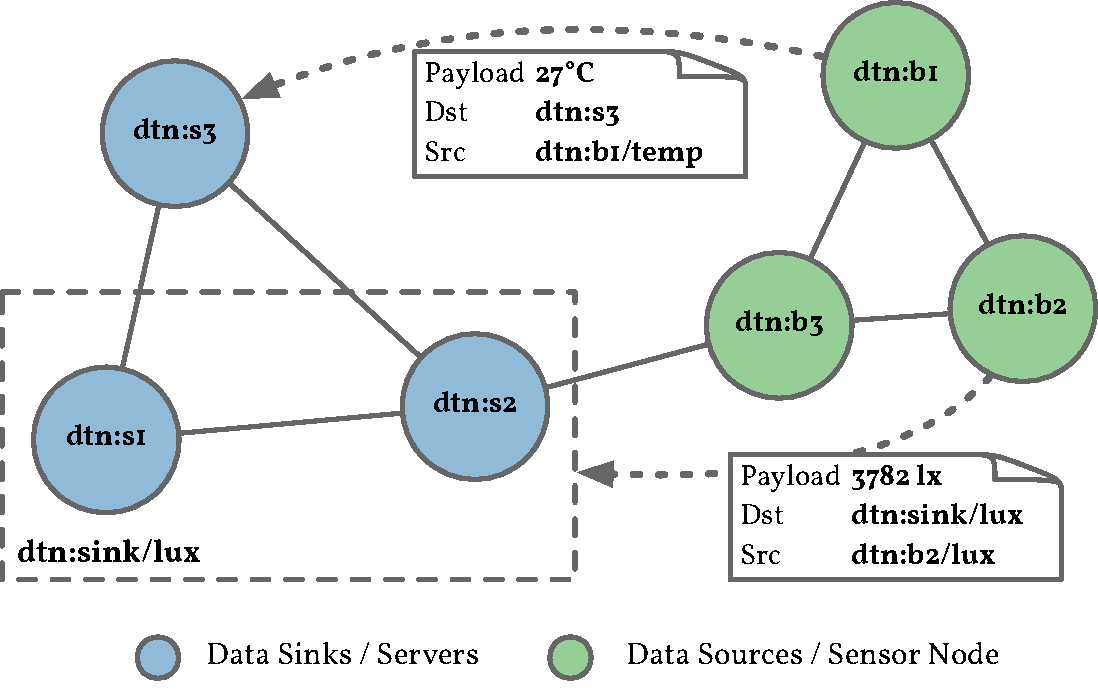
\includegraphics[width=0.75\linewidth,keepaspectratio]{include/nodes-endpoints}
  \end{figure}
\end{frame}

\subsection{Bundles and Blocks}

\begin{frame}
  \frametitle{Bundles and Blocks}

  \begin{itemize}
  \item \acs{BP7} packets are called Bundles
  \item A Bundle is a sequence of Blocks
  \item Binary represented in CBOR, RFC 7049
  \end{itemize}

  \begin{figure}
    \resizebox{\textwidth}{!}{
    \begin{tikzpicture}
    \begin{umlpackage}[fill=white]{Bundle}
      \umlclass[rectangle split parts=2, fill=white, visible on=<1>]{Primary Block}{
        Version: \texttt{7} \\
        Control Flags: \\
          \quad \textit{Status requested for reception} \\
        CRC Type: \textit{CRC32} \\
        Destination EID: \texttt{dtn:sink/lux} \\
        Source node EID: \texttt{dtn:b2/lux} \\
        Report-to EID: \texttt{dtn:b2/lux} \\
        Creation Timestamp: (\texttt{0}, \texttt{23}) \\
        Lifetime: \textit{3600000} \\
        CRC Value: \texttt{67 75 6D 6F}
      }{}
      \umlclass[rectangle split parts=2, visible on=<2>]{Primary Block}{
        Version: \texttt{7} \\
        Control Flags: \\
          \quad \textit{Status requested for reception} \\
        CRC Type: \textit{CRC32} \\
        Destination EID: \texttt{dtn:sink/lux} \\
        Source node EID: \texttt{dtn:b2/lux} \\
        Report-to EID: \texttt{dtn:b2/lux} \\
        Creation Timestamp: (\texttt{0}, \texttt{23}) \\
        Lifetime: \textit{3600000} \\
        CRC Value: \texttt{67 75 6D 6F}
      }{}
      \umlclass[rectangle split parts=2, fill=white, visible on=<3->]{Primary Block}{
        Version: \texttt{7} \\
        Control Flags: \\
          \quad \textit{Status requested for reception} \\
        CRC Type: \textit{CRC32} \\
        Destination EID: \texttt{dtn:sink/lux} \\
        Source node EID: \texttt{dtn:b2/lux} \\
        Report-to EID: \texttt{dtn:b2/lux} \\
        Creation Timestamp: (\texttt{0}, \texttt{23}) \\
        Lifetime: \textit{3600000} \\
        CRC Value: \texttt{67 75 6D 6F}
      }{}
      \umlclass[rectangle split parts=2, fill=white, x=4.75, y=1.054, visible on=<-2>]{Hop Count Block}{
        Type Code: \texttt{9} \\
        Number: \texttt{2} \\
        Control Flags: \textit{None} \\
        CRC Type: \textit{None} \\
        Data: (\texttt{64}, \texttt{42})
      }{}
      \umlclass[rectangle split parts=2, fill=white, x=8.6, y=1.054, visible on=<-2>]{Payload Block}{
        Type Code: \texttt{1} \\
        Number: \texttt{1} \\
        Control Flags: \textit{None} \\
        CRC Type: \textit{None} \\
        Data: \texttt{0E C6}
      }{}
      \umlclass[rectangle split parts=2, x=4.75, y=1.054, visible on=<3>]{Hop Count Block}{
        Type Code: \texttt{9} \\
        Number: \texttt{2} \\
        Control Flags: \textit{None} \\
        CRC Type: \textit{None} \\
        Data: (\texttt{64}, \texttt{42})
      }{}
      \umlclass[rectangle split parts=2, fill=white, x=4.75, y=1.054, visible on=<4>]{Hop Count Block}{
        Type Code: \texttt{9} \\
        Number: \texttt{2} \\
        Control Flags: \textit{None} \\
        CRC Type: \textit{None} \\
        Data: (\texttt{64}, \texttt{42})
      }{}
      \umlclass[rectangle split parts=2, x=8.6, y=1.054, visible on=<3->]{Payload Block}{
        Type Code: \texttt{1} \\
        Number: \texttt{1} \\
        Control Flags: \textit{None} \\
        CRC Type: \textit{None} \\
        Data: \texttt{0E C6}
      }{}
      \draw[decorate,decoration={brace,amplitude=10pt},xshift=-4pt,visible on=<3>]
        (10.5,-0.75) -- (3.1,-0.75) node [black,midway,yshift=-20pt]{Canonical Blocks};
    \end{umlpackage}
    \end{tikzpicture}
    }
  \end{figure}
\end{frame}

\subsection{Bundle Exchange}

\begin{frame}
  \frametitle{Bundle Exchange}

  \begin{itemize}
  \item Convergence Layer
    \begin{itemize}
    \item Transport technology for Bundles between nodes
    \item Implemented: TCP
    \item Possible: Bluetooth, LoRa, e-mail, bar code, \dots
    \end{itemize}

  \item Routing
    \begin{itemize}
    \item Selection of neighbors for Bundle delivery
    \item Implemented: DTLSR, Spray and Wait, Epidemic Routing
    \end{itemize}
  \end{itemize}
\end{frame}

\section{DTN7}

\subsection{Other \acs{DTN} components}

\begin{frame}
  \frametitle{Other \acs{DTN} components}

  \begin{itemize}
  \item Store for Bundles that are waiting for delivery
  \item RESTful API to dispatch and fetch Bundles
  \item Peer Discovery to detect nearby nodes
  \end{itemize}
\end{frame}

\subsection{DTN7 Architecture}

\begin{frame}
  \frametitle{DTN7 Architecture}

  \begin{figure}
    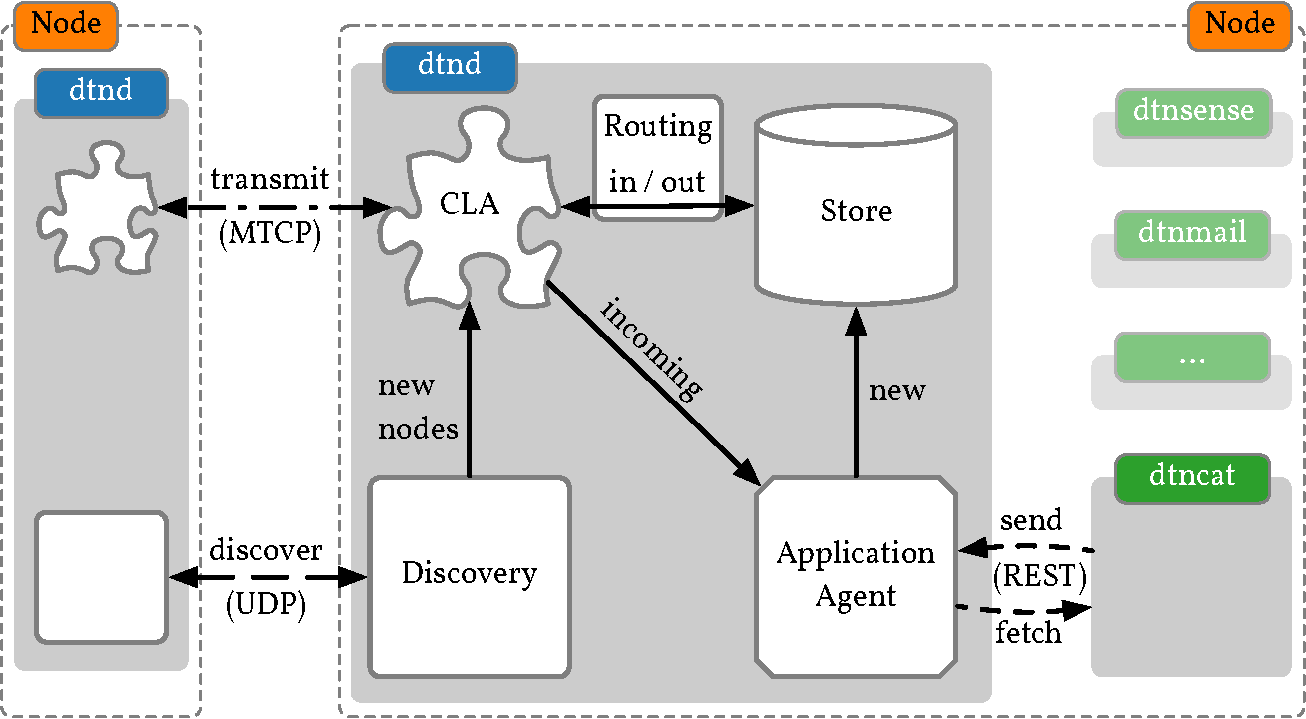
\includegraphics[width=\linewidth,keepaspectratio]{include/dtn7-architecture}
  \end{figure}
\end{frame}

\section{Evaluation}

\begin{frame}
  \frametitle{Evaluation}

  \begin{itemize}
  \item Up to 64 nodes emulated in the \acf{CORE}
  \item Nodes are connected pairwise in a chain topology
  \item Simulated IEEE 802.11g network, 54 MBit/s
  \end{itemize}

  \begin{figure}
    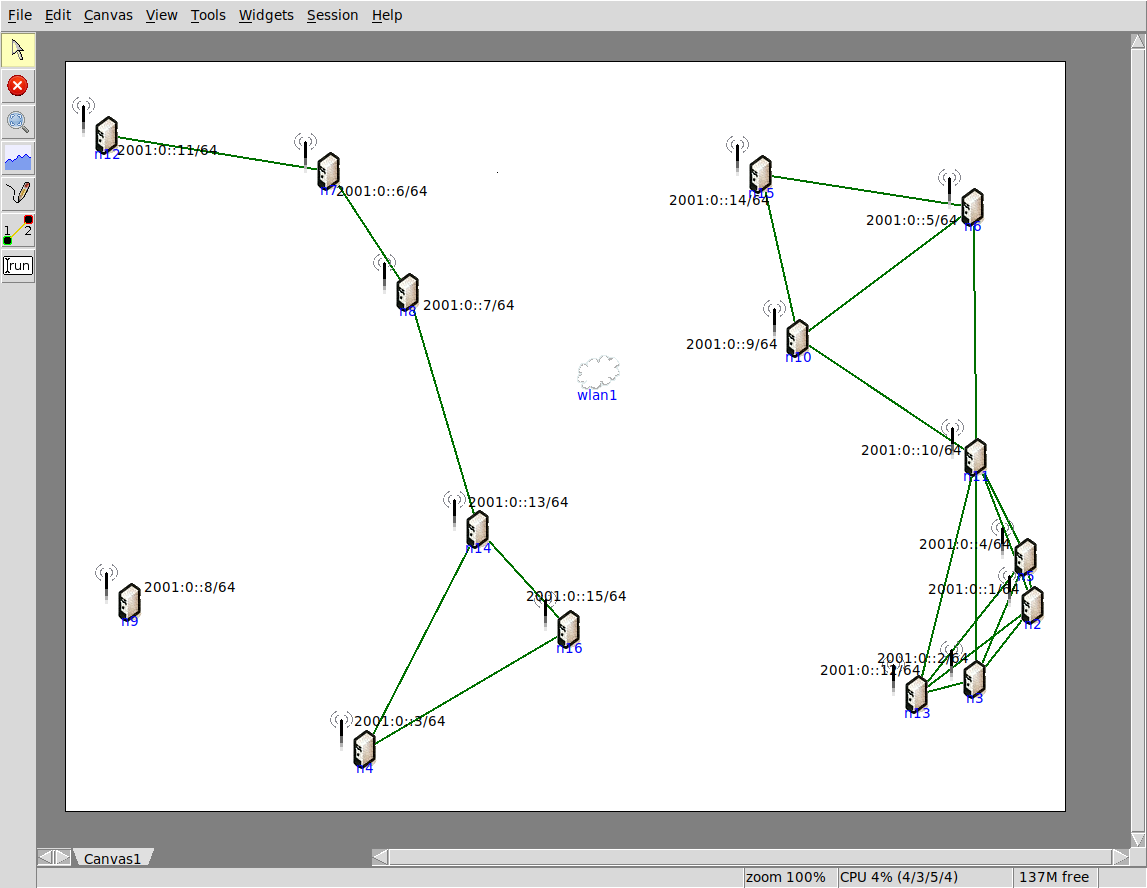
\includegraphics[width=0.6\linewidth,keepaspectratio]{include/core-screenshot}
  \end{figure}
\end{frame}

\begin{frame}
  \frametitle{Evaluation}

  \begin{itemize}
  \item Payload Size
  \begin{itemize}
    \item 64 KiB: compressed image
    \item 1 MiB: small image / short audio recording
    \item 5 MiB: smartphone image / audio recording
    \item 25 MiB: longer audio recording / short video
    \item 50 MiB: HD video
    \item 100 MiB: 4K smartphone video
  \end{itemize}
  \onslide<2>{
  \item{\acs{DTN} Software}
  \begin{itemize}
    \item DTN7
    \item Forban
    \item IBR-DTN
    \item Serval
  \end{itemize}
  }
  \end{itemize}
\end{frame}

\subsection{Results}

\begin{frame}
  \frametitle{Two nodes}

  \begin{figure}
    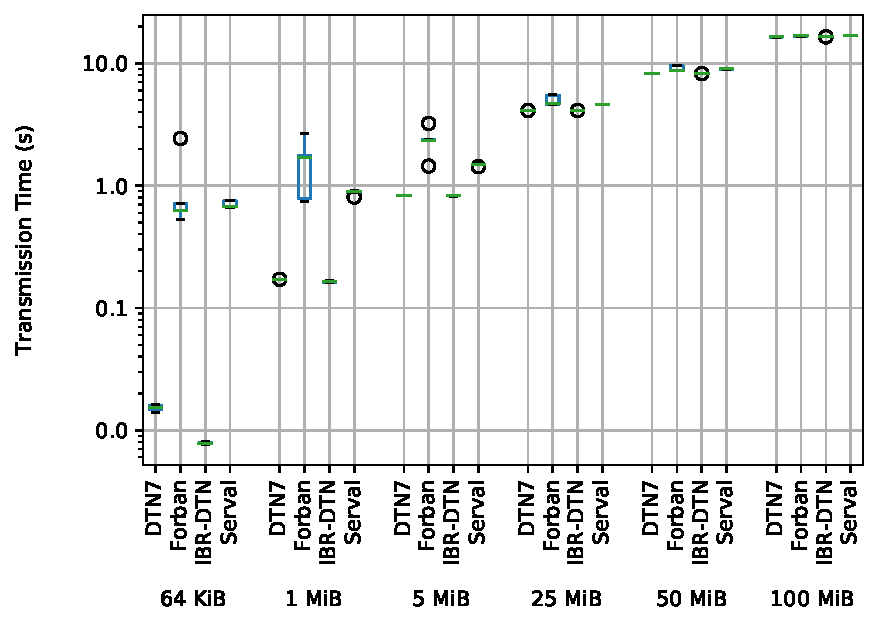
\includegraphics[width=\linewidth,keepaspectratio]{include/chain-runtimes-2}
  \end{figure}
\end{frame}

\begin{frame}
  \frametitle{64 nodes}

  \begin{figure}
    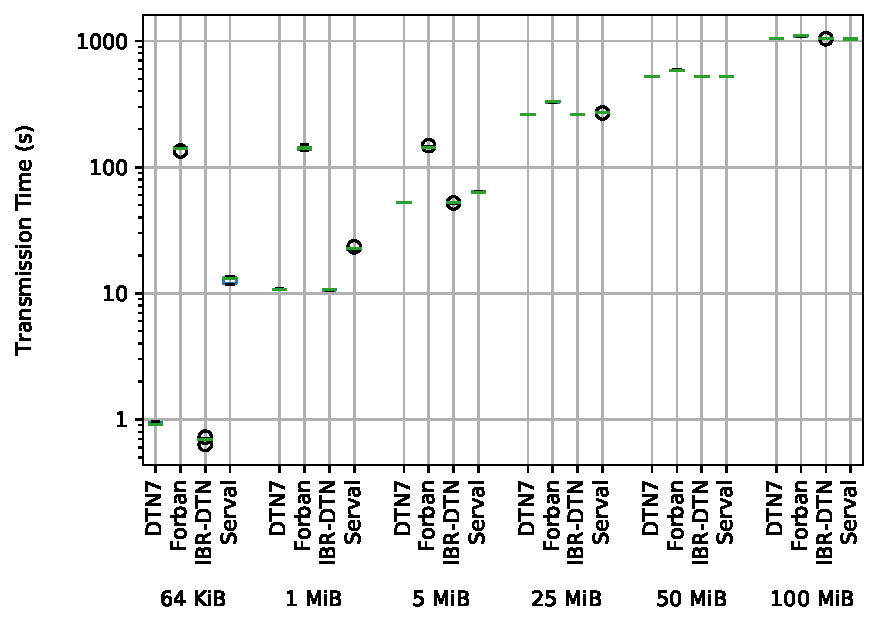
\includegraphics[width=\linewidth,keepaspectratio]{include/chain-runtimes-64}
  \end{figure}
\end{frame}

\section{End}

\begin{frame}[noframenumbering,plain]
\begin{center}
  \Large{DTN7}

  \large{An Open-Source Disruption-tolerant Networking \\ Implementation of Bundle Protocol 7}
\end{center}

\begin{center}
  \Large{https://dtn7.github.io/}
\end{center}
\end{frame}

\end{document}
